\chapter{Key-value stores}
A key-value store is a kind of non-relational database, which stores data as a
collection of key-value pairs where a key serves as a unique identifier.
\begin{figure}[h]
    \centering
    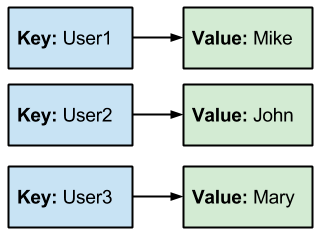
\includegraphics[width=.5\textwidth]{images/keyvalue.png}
    \caption{Basic concept of Key-Value}
\end{figure}

The main principle of the key-value store is not convenient for complex
interactions with the data because of its simple structure. In contrast this
type of databases saves resources. Because of their high performance key-value
stores are popular in real-time applications.

Representatives of key-value stores are \cite{dbkeyvalue}:

\begin{itemize}
    \item Redis
    \item Amazon DynamoDB
    \item Memcached
    \item Microsoft Azure Cosmos DB
    \item Hazelcast
\end{itemize}

\section{Essential Features}
\subsection{Simplicity}
In most cases there is no need for a relational database when developing a
simple application to manage basic data. Managing persons could be a typical
usage. Simplicity is an important keyword describing key-value databases. The
simple data model resembles a dictionary. Even the syntax for manipulating data
is straightforward. Regardless of the type of an operation, the user specifies a
name and a key to indicate the action performed on a key-value pair. An
elementary key-value database offers three operations:
\begin{itemize}
    \item Put: for adding or updating values
    \item Get: for getting a value by key
    \item Delete: for removing a key combined with its value
\end{itemize}
Another feature is the absence of types. Generally BLOBs can be stored, allowing
to put any data in there such as integers, strings, JSON, XML files or even
binary data like images. It’s up to the application to determine what type of
data is being used. Furthermore complex operations on data are expected to be
implemented by the application itself.

\subsection{Speed}
Due to the simplicity of key-value databases their internal operations are fast.
Internal design features can optimize performance as well. Data-intensive and
high-speed applications can be paired with these kind of databases but need to
calculate the results by themselves \cite{fulmanskikeyvalue}.
\newpage
\section{Limitations}
For key-value stores in general some limitations apply.
\begin{enumerate}
    \item The only way to look up values is querying the key.
    \item Range queries are not supported.
    \item There is no standard query language comparable to SQL within
    relational databases. In consequence queries from a key-value database may
    not be portable to another database.
\end{enumerate}
\cite{fulmanskikeyvalue}

